\normaltrue \difficilefalse \tdifficilefalse
\correctionfalse

%\UPSTIidClasse{11} % 11 sup, 12 spé
%\newcommand{\UPSTIidClasse}{12}

\exer{Disque $\star\star$ \label{B2:10:44}}
\setcounter{question}{0}\UPSTIcompetence[2]{B2-10}
\index{Compétence B2-10}
\index{Disque}
\ifcorrection
\else
\textbf{Pas de corrigé pour cet exercice.}
\fi




\ifprof
\else
Soit un secteur de disque de rayon $R$, d'épaisseur négligeable et de masse surfacique $\mu$. 
\begin{marginfigure}
\centering
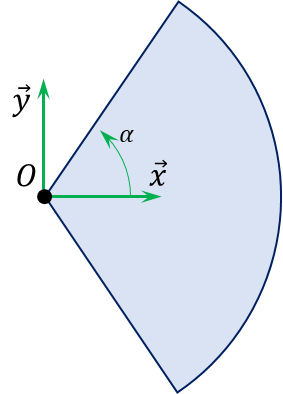
\includegraphics[width=\linewidth]{44_01}
\end{marginfigure}
\fi


\question{Déterminer la position du centre d'inertie $G$ du solide.}
\ifprof
\else
\fi

\question{Déterminer la matrice d'inertie du solide en $O$.}
\ifprof ~\\
\else
\fi


\ifprof
\else
\begin{flushright}
\footnotesize{Corrigé voir \ref{B2:10:44}.}
\end{flushright}%
\fi